\documentclass{beamer}
%\documentclass[aspectratio=169]{beamer}
%
\mode<presentation>
{
  \usetheme{default}      
  \usecolortheme{default}
  \usefonttheme{default} 
  \setbeamertemplate{navigation symbols}{}
  \setbeamertemplate{caption}[numbered]
} 

\usepackage[english]{babel}
\usepackage[utf8x]{inputenc}
\usepackage{pgfplots}
\pgfplotsset{compat=1.12}

\newcommand{\norm}[1]{\left\lVert#1\right\rVert}

\title[Classification]{Introduction to Machine Learning}
\subtitle{Lecture 4: Clustering}
\author{Alexis Zubiolo\newline\texttt{alexis.zubiolo@gmail.com}}
\institute{Data Science Team Lead @ Adcash}
\date{\today}

\begin{document}

\begin{frame}
  \titlepage
\end{frame}

\begin{frame}{What is clustering?}
\textbf{Clustering} algorithms aim at \textbf{grouping unlabeled objects}: In the datasets, we have $x$, but no $y$!
\vfill
\pause
\textbf{Goal}: Find clusters such that objects in the same cluster are more similar to each other than to objects in other clusters.
\pause
\vfill
Main \textbf{challenges}:
\begin{itemize}
	\item What does \textit{similar} mean?
	\item Given a similarity definition, how do we define clusters?
	\item How many clusters do we choose?
\end{itemize}
\end{frame}

\begin{frame}{Clustering: A few applications}
\textbf{Ecology}: Define comparisons of animal/plant communities over time
\vfill
\textbf{Web}: Recognize communities of users
\vfill
\textbf{Marketing}: Define groups of customers with similar behavior/interests to target them more efficiently
\vfill
\textbf{Image processing}: Segment images (\textit{e.g.} segment different tissues in biomedical imaging)
\vfill
And sometimes, we just have no label in our data, so clustering can be a good first approach to tackle some problems.
\end{frame}

\begin{frame}{Practical example: Image segmentation}
\centering
\begin{figure}
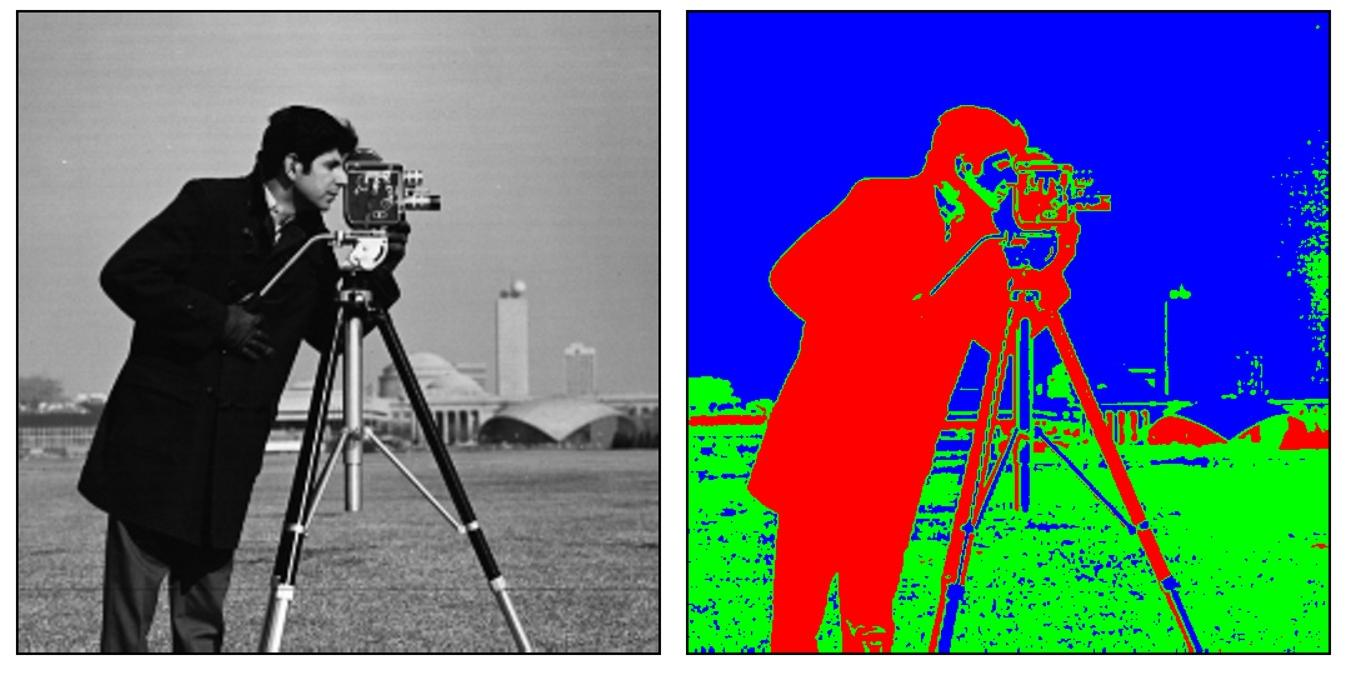
\includegraphics[width=\textwidth]{images/segmentation.jpg}
\end{figure}
Very basic example of image segmentation with clustering, just based on the intensity level.
\end{frame}

\begin{frame}{Course outline}
In this course, we will see 2 clustering algorithms:
\pause
\begin{itemize}
	\item $k$-means
	\item Hierarchical clustering
\end{itemize}
\end{frame}

\begin{frame}
	\center \Huge{$k$-means}
\end{frame}

\begin{frame}{$k$-means: Problem definition}
\textbf{Purpose}: Split the set of points into $k$ classes. $k$ is a \textbf{parameter}!
\pause
\vfill
We look for a partition $S = \left\{ S_1, S_2, \dots, S_k\right\}$ minimizing the within-cluster sum of squares.
\begin{equation*}
\min_S \sum_{i = 1}^{k} \sum_{x \in S_i} \norm{x - \mu_i}_2^2
\end{equation*}
\pause
where 
\begin{equation*}
\mu_i = \dfrac{1}{|S_i|} \sum_{x \in S_i} x
\end{equation*}
is the centroid (mean) of points in $S_i$.
\end{frame}

\begin{frame}{$k$-means: The algorithm}
$k$-means applies the following 2 iterations:
\pause
\begin{itemize}
	\item Define the \textbf{Voronoi diagram} generated by the $\mu_i$s:
	\begin{equation*}
		S_i^t = \left\{ x_p \mid \norm{x - \mu_i^t} \leq \norm{x - \mu_j^t}, 1 \leq j \leq k \right\}
	\end{equation*}
	\pause
	\item Update the centroid:
	\begin{equation*}
		\mu_i^{t+1} = \text{centroid}(S_i^t) = \dfrac{1}{S_i^t} \sum_{x \in S_i^t} x
	\end{equation*}
\end{itemize}
for all $i \in \left\{ 1, \dots, k\right\}$
\vfill
\pause
Problem in the above formulas: \textbf{initial value} for the $\mu_i$s?
\end{frame}

\begin{frame}{$k$-means: Initialization}
\textbf{Remark}: The $k$-means solution depends on the initial position of the $\mu_i$s centroids.

(see animation by Andrey Shabalin)
\vfill
\pause
2 related questions:
\begin{enumerate}
	\item How to choose the initial $\mu_i$s?
	\item How to have more stable results?
\end{enumerate}
\vfill
\pause
Unfortunately, no miracle strategy for Q1. A common strategy:
\begin{itemize}
	\item Several $k$-means with random initializations
	\item Majority vote
\end{itemize}
\end{frame}

\begin{frame}{Speeding up $k$-means}
Each $k$-means iteration is done over all the points in the dataset. This can be computationally expensive, especially if
\begin{itemize}
	\item There are many points
	\item The point density is big
\end{itemize}
What to do to \textbf{speed up the process}?
\pause
\vfill
\textbf{Alternative}: \textbf{Mini-batch} $k$-means. At each iteration
\begin{itemize}
	\item Choose a subset of points
	\item Apply a $k$-means iteration 
\end{itemize}
\end{frame}

\begin{frame}{Number of clusters}
In some applications, you know how many clusters you want. In this case, $k$ is \textbf{easy to set}.
\vfill
In other applications, we don't know the optimal number of classes we want. Ideally, we would like $k$ to be \textbf{selected automatically}.
\vfill
There is always \textbf{some ambiguity} in selecting the \textit{optimal} number of clusters. This is normal: When doing unsupervised learning, there is necessarily some \textbf{inherent subjectivity} in the labeling process!
\end{frame}

\begin{frame}{Number of clusters}
That being said, it is possible to define some criterias to determine whether $k_1$ is a better number of clusters than $k_2$. We can use the sum of squared errors to the centroids:
\begin{equation*}
\text{SSE}(k) = \sum_{i = 1}^{k} \sum_{x \in S_i} \norm{x - \mu_i}_2^2
\end{equation*}
And apply the \textbf{Elbow method}.
\vfill
\pause
Note that this is not a miracle solution.
\end{frame}

\begin{frame}{The elbow rule/method}
\begin{figure}
\centering
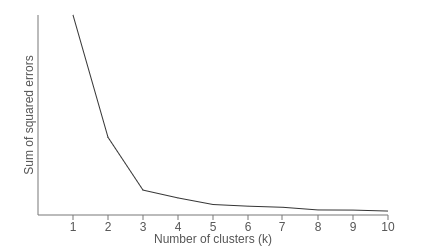
\includegraphics[width=\textwidth]{images/elbow.png}
\end{figure}
\end{frame}

\begin{frame}{$k$-means: concluding remarks}
Pros:
\begin{itemize}
	\item Fast, and can be faster with mini-batches
	\item Intuitive and easy to implement
\end{itemize}
\vfill
\pause
Cons:
\begin{itemize}
	\item Might not always give the same solution
	\item Number of clusters $k$
\end{itemize}
\vfill
\pause
We can use different metrics to link clusters and various linkage criteria. (More on this later.)
\end{frame}

\begin{frame}
	\center \Huge{Hierarchical clustering}
\end{frame}

\begin{frame}{Hierarchical clustering}
\textbf{Bottom-up} approach:
\begin{itemize}
	\item \textbf{Bottom}: Initially, each point is a cluster
	\item \textbf{Top}: Merge the 2 closest clusters until we have one cluster
\end{itemize}
\vfill
\pause
\textit{closest} has to be defined. We can use the \textbf{Euclidean norm}: $a$ and $b$ are closer than $a'$ and $b'$ if and only if $\norm{a - b} \leq \norm{a' - b'}$.
\pause
\vfill
(illustration on the clipboard)
\end{frame}

\begin{frame}{Hierarchical clustering: Dendograms}
\begin{tikzpicture}[sloped]
\node (a) at (-6,0) {a};
\node (b) at (-3,0) {b};
\node (c) at (-0.5,0) {c};
\node (d) at (0.5,0) {d};
\node (e) at (2,0) {e};
\node (ab) at (-4.5,3) {};
\node (cd) at (0,1) {};
\node (cde) at (1,2) {};
\node (all) at (-1.5,5) {};
\draw[->] (-7,0) -- node[above]{distance} (-7,6);

\pause
\draw  (c) |- (cd.center);
\draw  (d) |- (cd.center);
\pause
\draw  (e) |- (cde.center);
\draw  (cd.center) |- (cde.center);
\pause
\draw  (a) |- (ab.center);
\draw  (b) |- (ab.center);
\pause
\draw  (ab.center) |- (all.center);
\draw  (cde.center) |- (all.center);

\pause
\draw[dashed, thick, red] (-6.5,2.5) -- (+2.5,+2.5);
\pause
\draw[dashed, thick, blue] (-6.5,3.5) -- (+2.5,+3.5);
\pause
\draw[<-] (+3,0) -- node[below]{number of clusters} (+3,6);
\end{tikzpicture}
\vfill
\pause
Formally, this can be done with a \textbf{linkage criterion}.
\end{frame}

\begin{frame}{Hierarchical clustering: concluding remarks}
Pros:
\begin{itemize}
	\item No need to provide an initial number of classes
	\item Can split the clusters at different levels
\end{itemize}
\vfill
\pause
Cons:
\begin{itemize}
	\item Similarity matrix (need to compute the distances between all pairs of points in the dataset): Does not scale well with the number of points!
\end{itemize}
\vfill
\pause
We can use different metrics to link clusters and various linkage criteria.
\vfill
\pause
Top-down approach also possible.
\end{frame}

\begin{frame}{Conclusion}
Clustering methods create groups within a set of unlabeled points.
\vfill
\pause
They typically rely on:
\begin{itemize}
	\item A similarity (or dissimilarity) measure (\textit{e.g.} the Euclidian norm)
	\item A few parameters, \textit{e.g.}
	\begin{itemize}
		\item The number of clusters for $k$-means
		\item The dendogram cut (linkage) for hierarchical clustering
	\end{itemize}
\end{itemize}
\end{frame}

\begin{frame}
	\center
	\huge{Thank you! Questions?}
\end{frame}

\end{document}